\begin{frame}[t]{A Theory of Onset Temperature in 2D: The KTHNY Melting Scenario}

\begin{figure}
\begin{overprint}

\onslide<2-4>\centering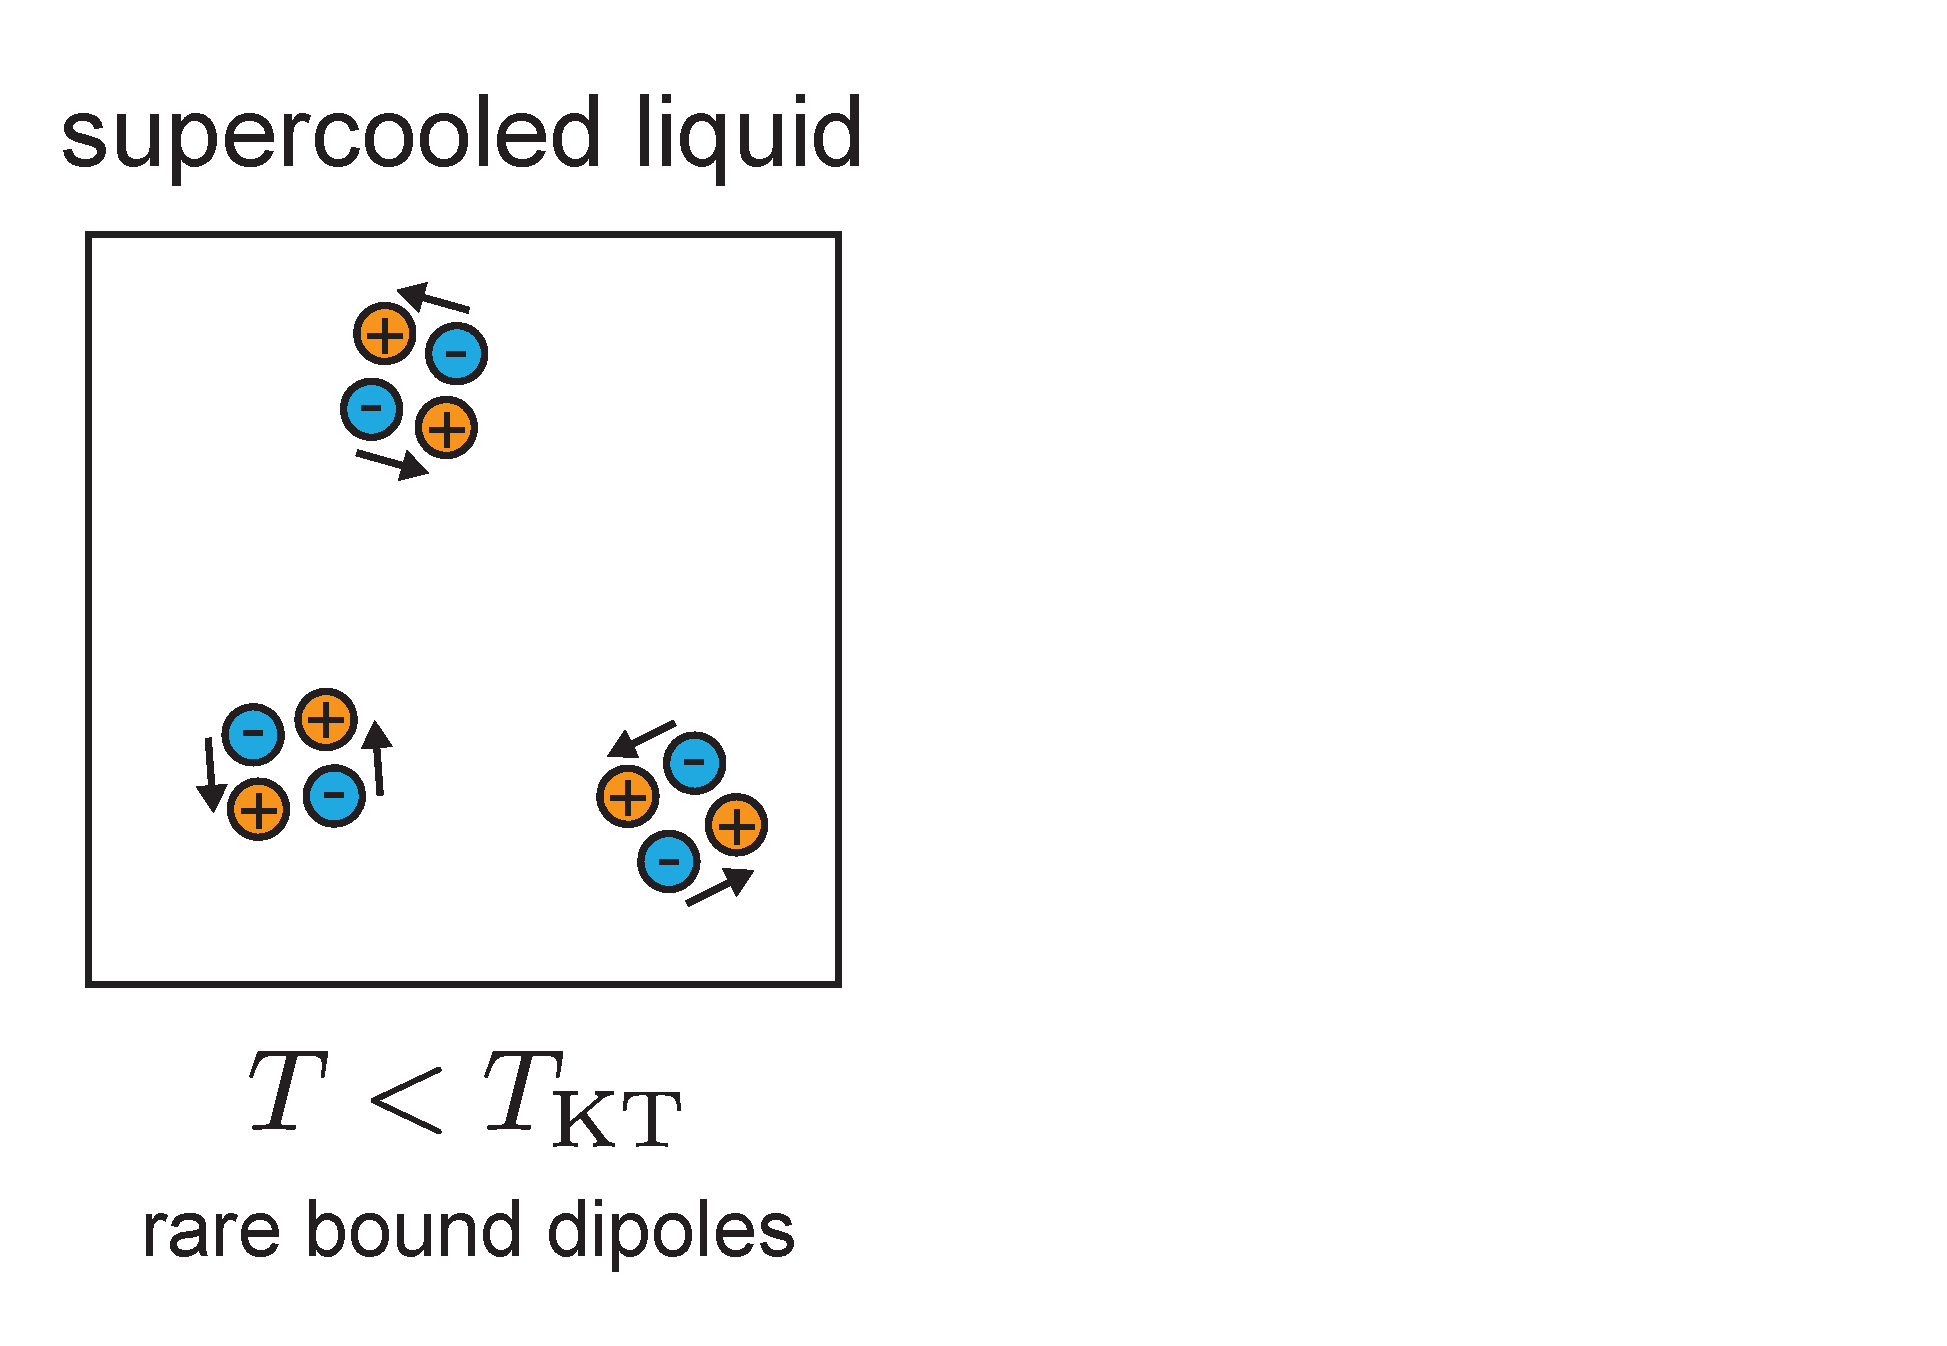
\includegraphics[height=0.675\textheight]{c.7-kt_meltingscenario/mechanism-0.pdf}%\caption{Testing}

\onslide<5->\centering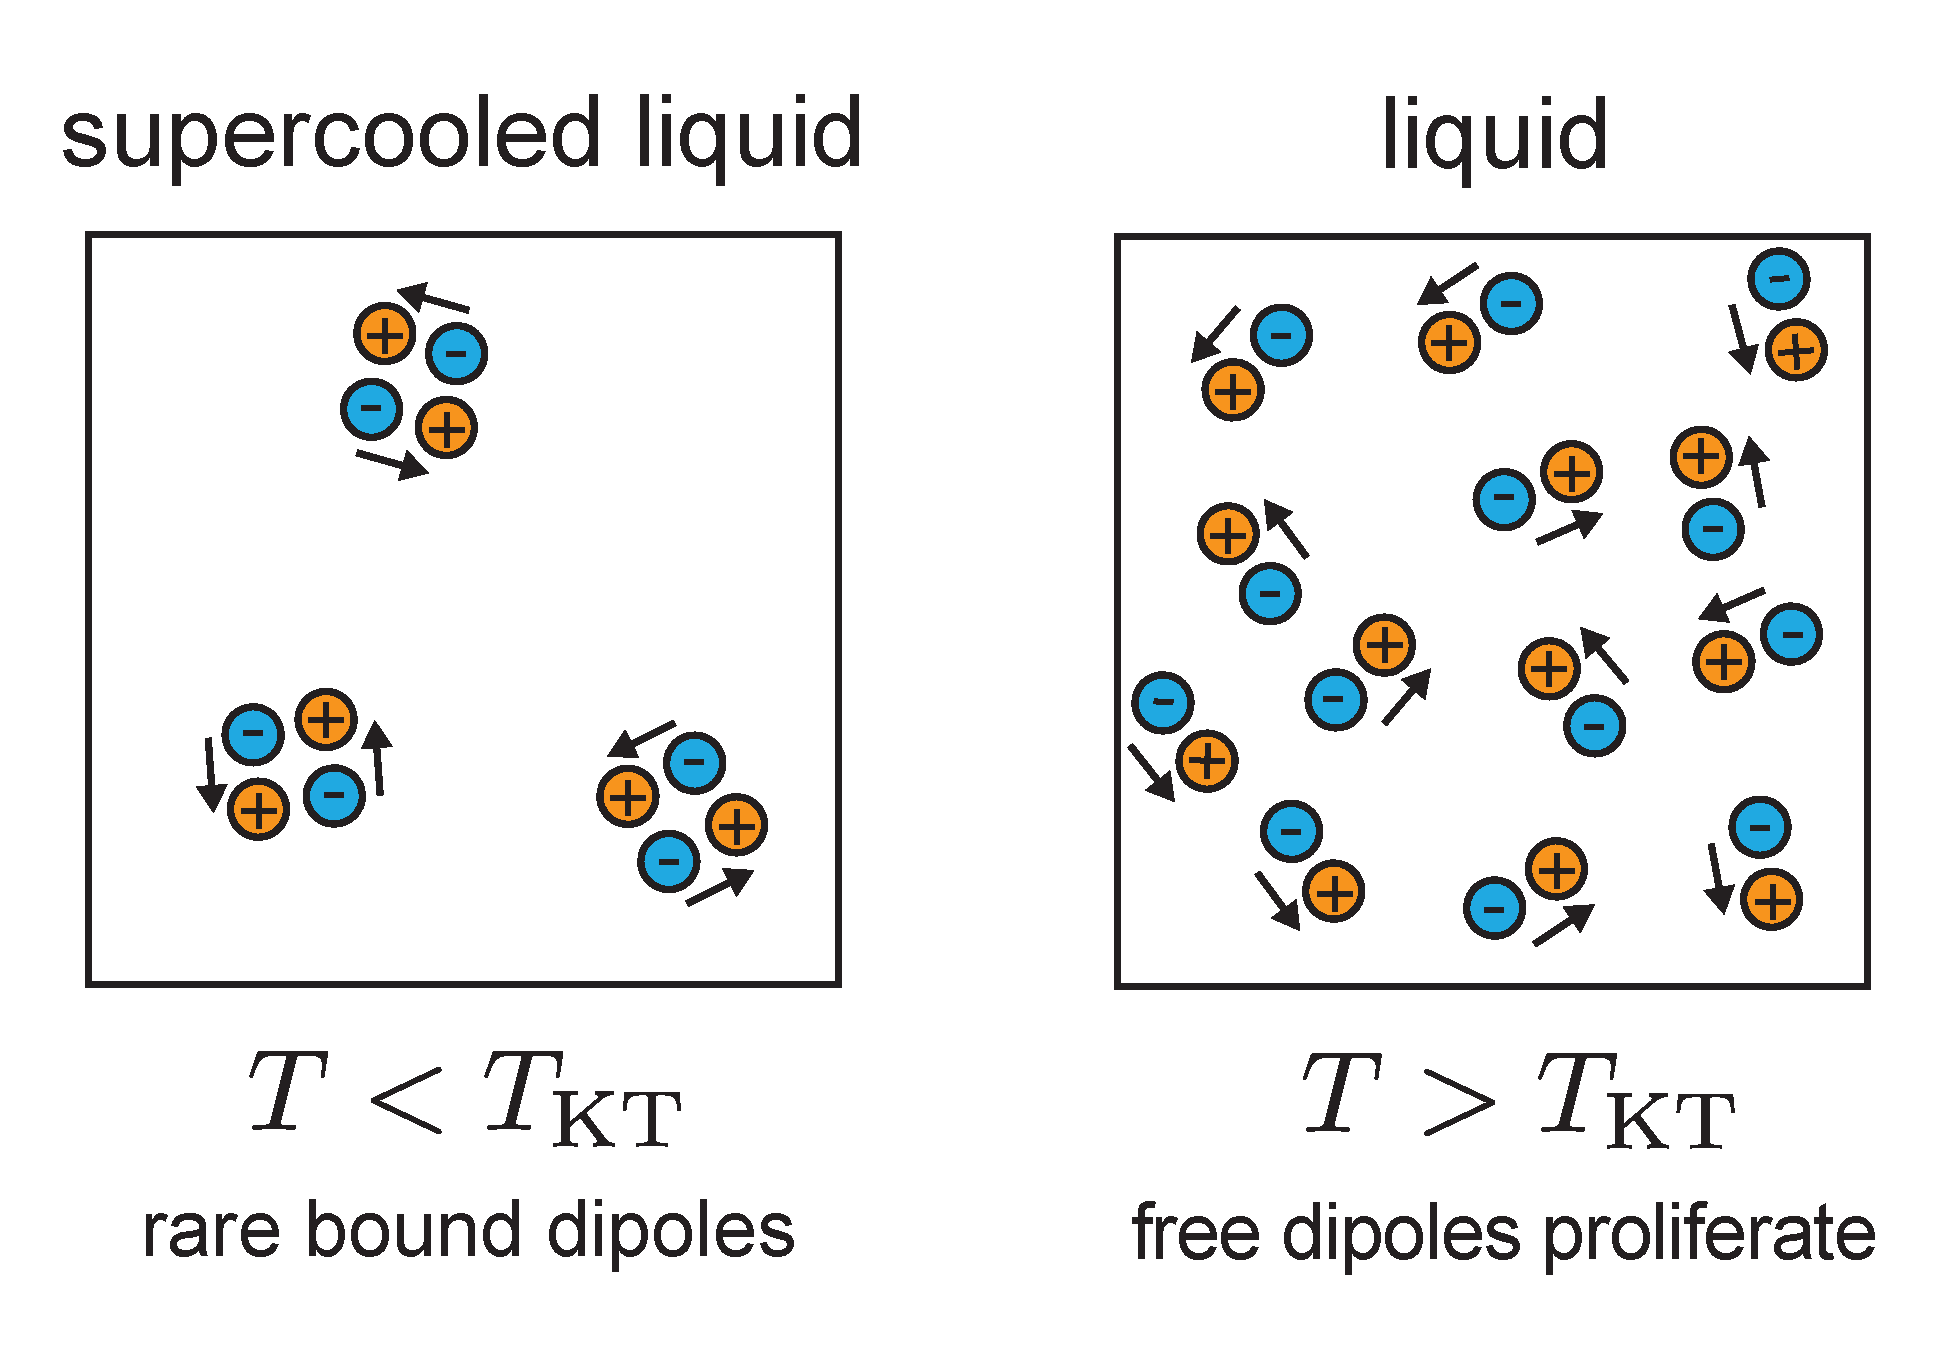
\includegraphics[height=0.675\textheight]{c.7-kt_meltingscenario/mechanism-1.pdf}%\caption{Testing}

%\onslide<4->\centering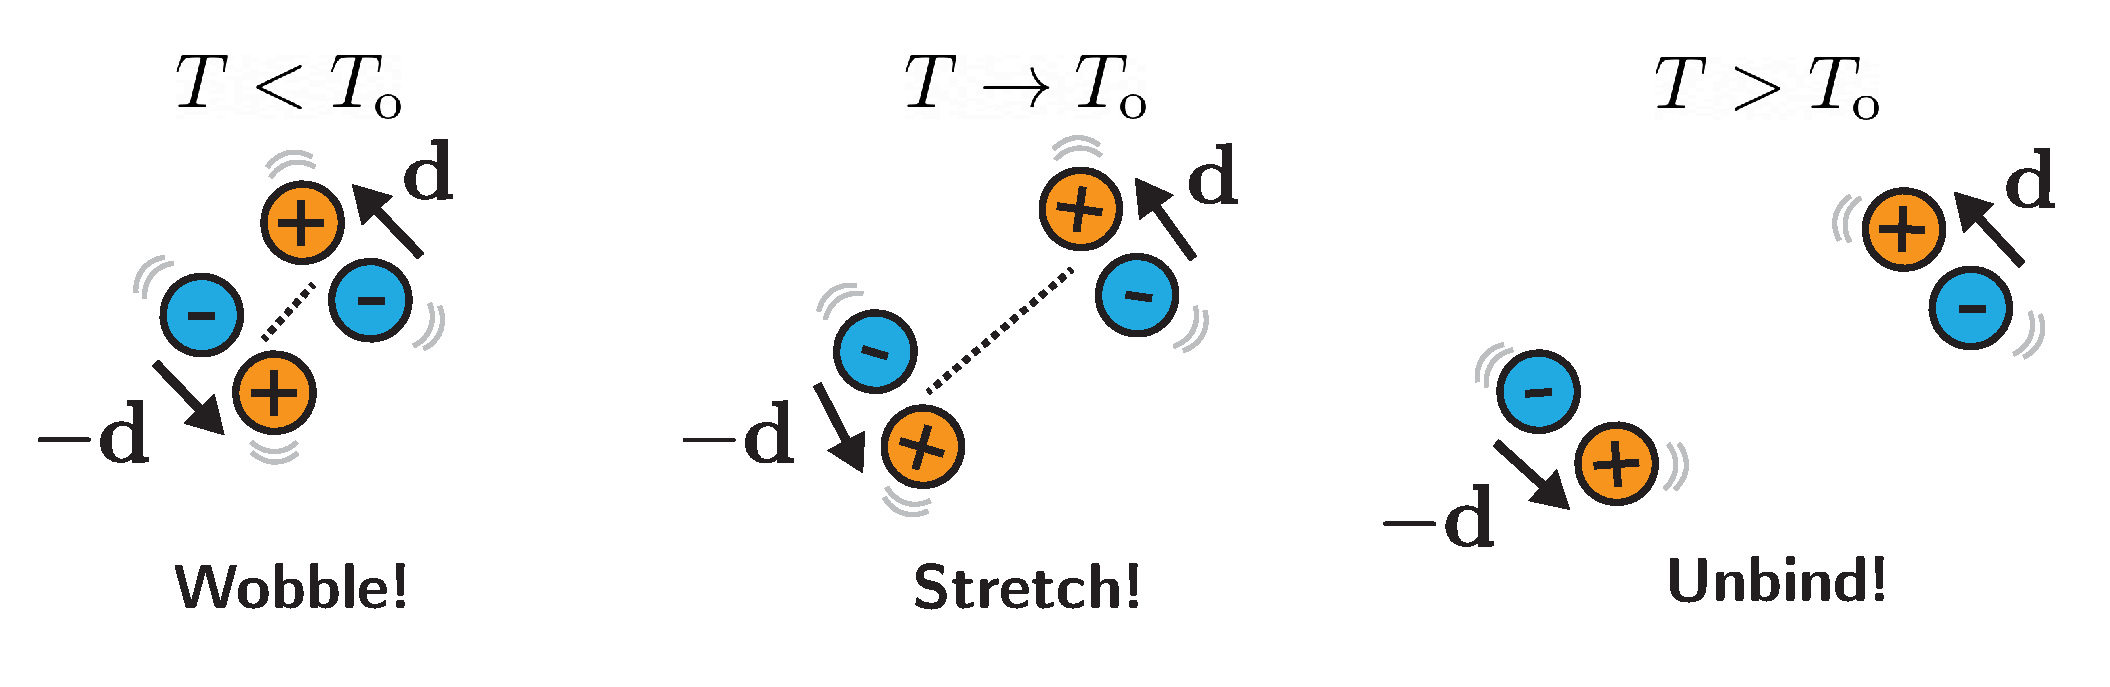
\includegraphics[width=0.925\linewidth]{slide_13/dofs_quadrupole-3.pdf}
% \begin{columns}
% \begin{column}{0.5\linewidth}
% \begin{itemize}
%     \item T
% \end{itemize}
% \end{column}

% \begin{column}{0.5\linewidth}

\end{overprint}
    
\end{figure}

\vspace{-10pt}

\only<1-7>{
\begin{itemize}
\item<2-> \textbf{$T < T_\mathrm{KT}$:} Rare localized pure-shear excitations \onslide<3->{$\to$ a (defected) solid at intermediate timescales} \onslide<4->{$\to$ \textbf{a renormalized shear modulus} $\km{G^\mathrm{R}} < G^\mathrm{IS}$.}
\item<5-> \textbf{$T > T_\mathrm{KT}$:} Proliferation of free dipoles \onslide<6->{$\to$ \textbf{entropy} drives the system to behave as a fluid}\onslide<7->{$\to$ vanishing renormalized shear modulus $\km{G^\mathrm{R}} =0$}

%\only<6->{$\to$ similar to the Kosterlitz-Thouless-Halperin-Nelson-Young (KTHNY) theory.}
%\footnote{Kosterlitz and Thouless, \textit{J. Phys. C} (1972); Kosterlitz and Thouless, \textit{J. Phys. C} (1973); Halperin and Nelson, \textit{Phys. Rev. Lett.} (1978); Nelson, \textit{Phys. Rev. B} (1978); Nelson and Halperin, \textit{Phys. Rev. B} (1979); Young, \textit{Phys. Rev. B} (1979)}}

\end{itemize}
}
\only<8->{
\begin{block}{\Large \centering The Task}
Determine the temperature $T_\mathrm{KT}$ where $\beta_\mathrm{KT} \km{Y^\mathrm{R}(T=T_\mathrm{KT})} d_\mathrm{c}^2 = 16 \pi$ due to unbinding of localized excitations $\to$ Compare predicted $T_\mathrm{KT}$ to observed the onset temperature $T_\mathrm{o}$!
\end{block}
}

% \end{column}

% \end{columns}


    
\end{frame}